% Diagram: System architecture — 3 components with a data flow.
% Coordinates: (x, y)
%   input   at (-4, 0) -- left
%   process at  (0, 0) -- center
%   output  at  (4, 0) -- right
%   storage at  (0,-2) -- below, persistence
%
% Embeds P1 (explicit dims), P2, P4 (directional labels).
\documentclass[border=4pt]{standalone}
\usepackage{tikz}
\usetikzlibrary{positioning, arrows.meta, calc, shapes.geometric, shapes.misc}
\begin{document}
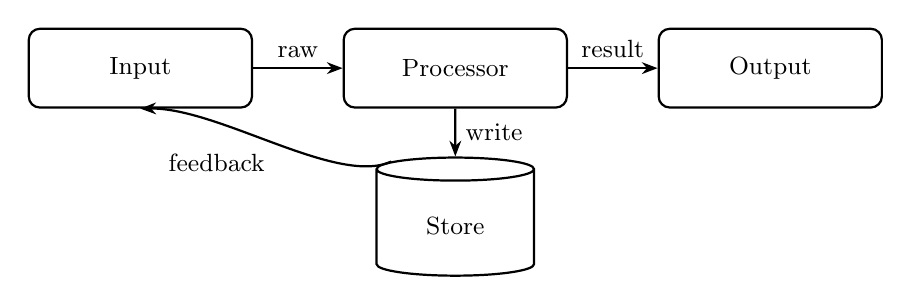
\begin{tikzpicture}[
    every node/.style={font=\small},
    block/.style={draw, rounded corners,
                  minimum width=2.8cm, minimum height=1cm,
                  text width=2.6cm, align=center, thick},
    store/.style={draw, cylinder, shape border rotate=90, aspect=0.3,
                  minimum width=2cm, minimum height=1.5cm, thick},
    arrow/.style={-{Stealth[length=2mm]}, thick}
  ]
  \node[block] (input)   at (-4, 0)  {Input};
  \node[block] (process) at (0, 0)   {Processor};
  \node[block] (output)  at (4, 0)   {Output};
  \node[store] (storage) at (0, -2)  {Store};

  \draw[arrow] (input)   -- (process) node[midway, above] {raw};
  \draw[arrow] (process) -- (output)  node[midway, above] {result};
  \draw[arrow] (process) -- (storage) node[midway, right] {write};
  \draw[arrow] (storage.north west) .. controls (-1.5, -1.5) and (-3, -0.5) .. (input.south)
        node[midway, below left] {feedback};
\end{tikzpicture}
\end{document}
